\chapter{Experiments}
The evolutionary algorithms described in section \ref{evolution-strategies} were implemented in C++. This language was chosen due to its flexibility, performance and the possibility to make use of the ngSPICE simulator. The implementation also utilizes the RInside library which integrates R into C++. The R language is used to plot graphs dynamically during the evolution either to the screen or to a file so the user can see and record how the solution evolves.\\
The program is written as a console application and the user can specify the properties of the evolution via command-line arguments. This approach also allows the user to easily run the application multiple times and collect the results of the evolution.\\
The results are in the form of graphs and a text output which contains the details about the evolution run. The graphs can be either dynamically generated to the screen during the program run or saved as files to the local drive as well as the text output. The user can specify how often the graphs and text description are generated, for example, each time when the fitness function of the best chromosome in the population changes by 1\%.

\section{Chromosomes evaluation} \label{chromosomes-evaluation}
A fitness function provides us means by which we can determine how good the evolved solution is so that we can distinguish the more appropriate candidates from the less appropriate ones. It is important to mention that the quality of this function is essential because the ability of the algorithm to find the most suitable solution is highly dependent on the ability of the fitness function to distinguish between the individuals. The value of the function is a positive real number in our case and the algorithm uses it only for comparing the individuals between each other. We consider those individuals with the lower value as the better ones.\\
The implementation required some methods of trial and error and in the end, there are three fitness functions implemented in this thesis. All of them use the ngSPICE simulator in order to obtain the output of the amplifier and assess it afterwards. The simulation is done for every candidate solution and it takes most of the computation time of the overall evolutionary algorithm.

\subsection{Best match with the reference solution}
This fitness function has been implemented as the first one in order to find out if the evolution has at least the ability to get close to the analytical solution. It is based on the method of least squares which is used in regression analysis.\\
    The fitness function uses the output voltage vector from the simulator for assessing the chromosomes. The vector represents the waveform of the output signal from the circuit and the shape of the waveform gets similar to an inverted sine wave as the solution evolves. The length of the vector is set to 69 (the sampling period is approximately \SI{20}{\micro\second}) elements during the whole evolution and the vector contains approximately 2.5 periods of the signal (the signal's frequency is \SI{20}{\kilo\hertz}). The fitness function uses two types of these vectors, one serves as the reference vector (the output of the amplifier which elements' values were calculated analytically) and all the candidate vectors are compared to it. As we can see in figure \ref{ce-amplifier-sim}, the first period of the signal is unstable, so the fitness function skips it and picks only the second period for comparison with the reference signal. It is sufficient to compare only the second period because the shape of the signal doesn't change anymore after the circuit gets to a stable state.\\
    The functions in algorithm \ref{get-second-period} are used to extract the second period from the waveform. Since the vector has a constant length and the values represent an inverted sine wave, we can walk through the first two and the last half-period to get to the desired part of the signal. When the evolution starts, the waveform of some candidate solutions is not in the shape of an inverted sine wave and therefore it crosses zero sooner than the desired waveform. In this case, the algorithm ends with indexes close to the starting and ending index and such candidate solution is assessed with a high fitness value.

    \begin{algorithm}
    \caption{Find the first and last index of the second period}
    \label{get-second-period}
    \begin{algorithmic}[1]
        \Function{getStart}{$vector$}
            \State $start \gets 0$;
            \While{$start < 0$}
                \State $start \gets start + 1$;
            \EndWhile
            \While{$start > 0$}
                \State $start \gets start + 1$;
            \EndWhile
            \State \Return $start$;
        \EndFunction

        \Function{getEnd}{$vector$}
            \State $end \gets vector.length()$;
            \While{$end < 0$}
                \State $end \gets end - 1$;
            \EndWhile
            \State \Return $end$;
        \EndFunction
    \end{algorithmic}
    \end{algorithm}

    The function in algorithm \ref{bestFit} is used to evaluate the candidate solutions. It iterates over the second period in both reference and candidate vectors and it calculates the sum of squares which sides are defined by the difference between the values in the reference vector and the candidate vector. The overall sum is returned as the result of the fitness function and the lower the value, the better the candidate solution is. The reason why we add up squares and not only the absolute values of the differences is important. Consider two imaginary vectors of two values which differ from the reference vector by $(1, 5)$ and by $(3,3)$. The sum of the absolute values is 6 in both cases, so this method doesn't distinguish between these vectors. However, the sum of the squares is 26 for the first vector and 18 for the second one. This difference is important as we want all the values to be close to the reference and not only some of them and therefore the second vector is assessed as a better one.

\begin{algorithm}
\caption{Fitness evaluation using the analytical solution}
\label{bestFit}
\begin{algorithmic}[1]
    \Function{rateChromosome}{$candidateVector$, $referenceVector$}
        \State $fitness \gets 0$;
        \State $start \gets$ \Call{getStart}{$candidateVector$};
        \State $end \gets$ \Call{getEnd}{$candidateVector$};
        \For{$i \gets start : end$}
            \State $fitness \gets fitness + (referenceVector[i] - candidateVector[i])^2$;
        \EndFor
        \State \Return $fitness$;
     \EndFunction
\end{algorithmic}
\end{algorithm}

We can see the result of the evolution using this fitness function in figure \ref{best-match}.

\begin{figure}[H]
    \centerline{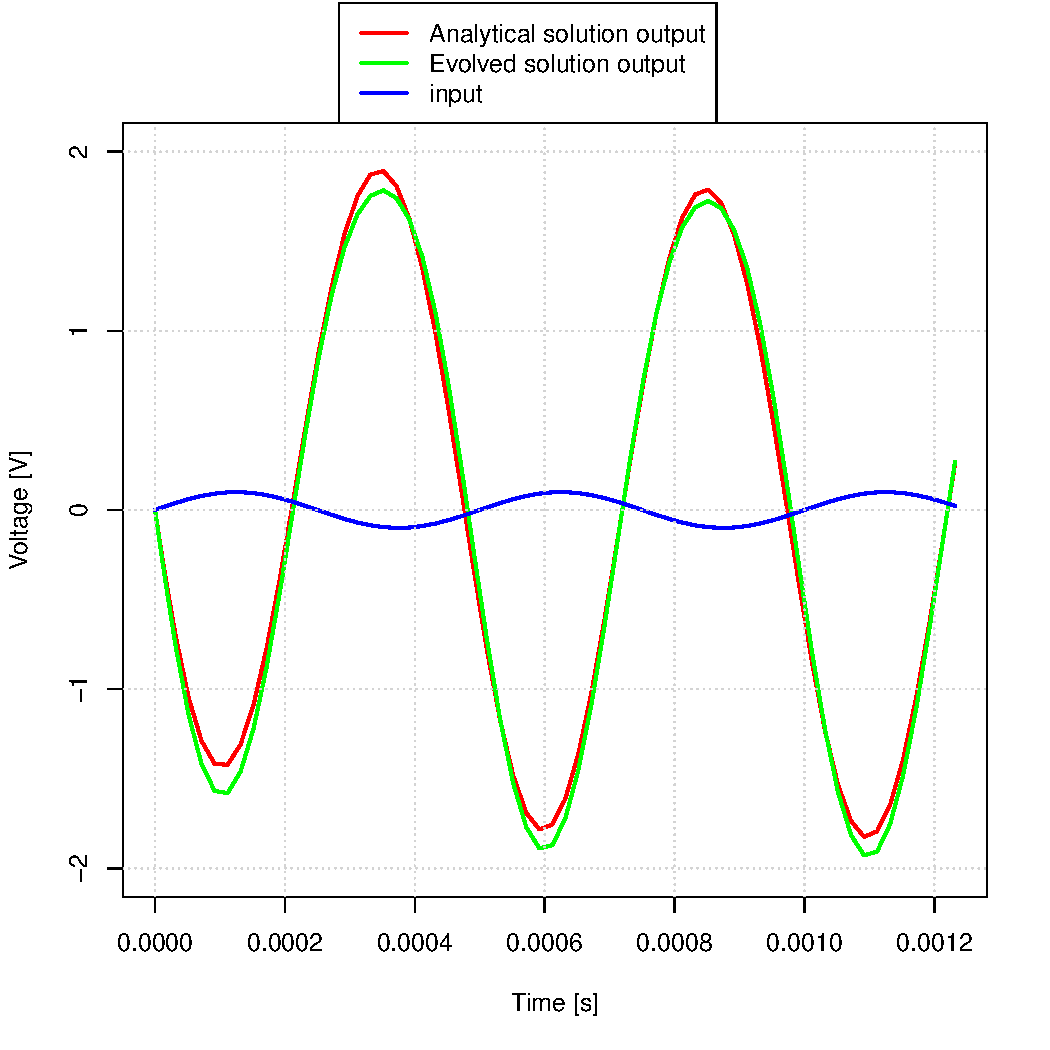
\includegraphics[scale=0.6]{best-match}\label{best-match}}
    \caption{The result of evolution towards the analytical solution}
\end{figure}

\subsection{Ideal sine wave}
This method is similar to the previous one but instead of using the pre-simulated output as a reference, it uses an analytically calculated sine wave. An analytical sine wave is used in order to force the evolution towards such solution that won't produce a distorted output signal since the input is in the form of a sine wave as well. The function also uses the method of least squares explained in the previous section and it iterates over the second period of the signal which is represented by the $candidateVector$.\\
We can see the technique in algorithm \ref{idealSine}. In every iteration, it calculates the value of the sine wave and compares it with the simulated signal. The sum of the comparisons is then returned as the fitness value and the lower the result is, the closer the candidate solution is to the reference. The amplitude of the sine wave is set by the user, so this method allows users to design amplifiers with an arbitrary amplification which doesn't exceed the circuit's capabilities.

\begin{algorithm}
\caption{Fitness evaluation using the ideal sine wave}
\label{idealSine}
\begin{algorithmic}[1]
    \Function{rateChromosome}{$candidateVector$, $amplitude$}
        \State $fitness \gets 0$;
        \State $start \gets$ \Call{getStart}{$candidateVector$};
        \State $end \gets$ \Call{getEnd}{$candidateVector$};
        \State $refSineSize \gets end - start$;
        \For{$i \gets 0 : refSineSize$}
           \State \scalebox{1.3}{$refSine \gets -amplitude \cdot \sin(\frac{2 \pi i}{refSineSize - 1})$};
           \State $fitness \gets fitness + (refSine - candidateVector[start + i])^2$;
        \EndFor
        \State \Return $fitness$;
    \EndFunction
\end{algorithmic}
\end{algorithm}

\subsection{Maximal amplitude}
This fitness function is designed to rate the candidate solutions only according to the amplitude of the output regardless of the waveform's shape. It can be used for finding the highest amplification capabilities of the circuit. The function finds the trough and the peak in the second amplitude and returns the multiplicative inverse of their difference.

\begin{algorithm}
\caption{Rating the chromosomes according to the amplitude}
\label{maxAmp}
\begin{algorithmic}[1]
    \Function{rateChromosome}{$candidateVector$}
        \State $start \gets$ \Call{getStart}{$candidateVector$};
        \State $end \gets$ \Call{getEnd}{$candidateVector$};
        \State $trough \gets \min(candidateVector[start]$, $candidateVector[end])$;
        \State $peak \gets \max(candidateVector[start]$, $candidateVector[end])$;
        \State \Return \scalebox{1.2}{$\frac{1}{peak - trough}$};
    \EndFunction
\end{algorithmic}
\end{algorithm}

\subsection{Waveform symmetry}
All of the fitness functions discussed above have difficulties in finding symmetrical waveforms. An example is shown in figure \ref{asymmetrical-ideal-sine}.

\begin{figure}[H]
    \centerline{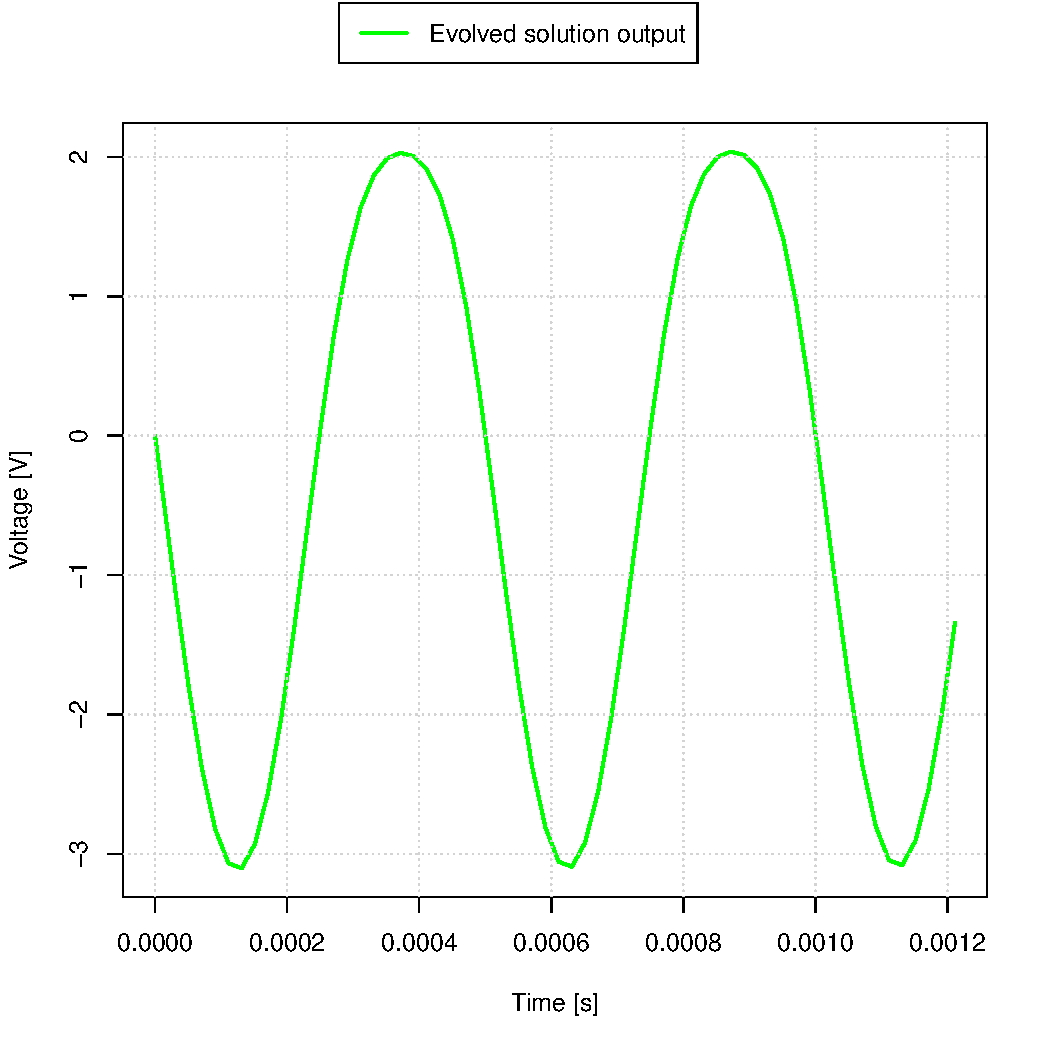
\includegraphics[scale=0.6]{asymmetrical-ideal-sine}\label{asymmetrical-ideal-sine}}
    \caption{An asymmetrical result of the evolution using the 'ideal sine wave' evaluation}
\end{figure}

The problem is that at the start, the output signal has zero power and as the evolution continues, only one half of the signal rises and the fitness function value decreases even though the evolution doesn't go in the right direction. At the end, the evolution ends up in the state shown in figure \ref{asymmetrical-ideal-sine}. The first solution to this problem is described in formula \ref{sym1}.

\begin{equation} \label{sym1}
result = (|peak + trough| + 1) \cdot fitness
\end{equation}

The $peak$ and $trough$ values are obtained in the same way as in algorithm \ref{maxAmp}. If the signal is symmetrical, the absolute value of the sum of these values is close to zero and therefore the $result$ will also be lower. We add 1 to the sum because we need to distinguish between perfectly symmetrical signals with different fitness. However, it emerged that this approach is too restrictive as it promotes only signals which are perfectly symmetrical, but often distorted. The result is shown in figure \ref{symmetrical-ideal-sine}.

\begin{figure}[H]
    \centerline{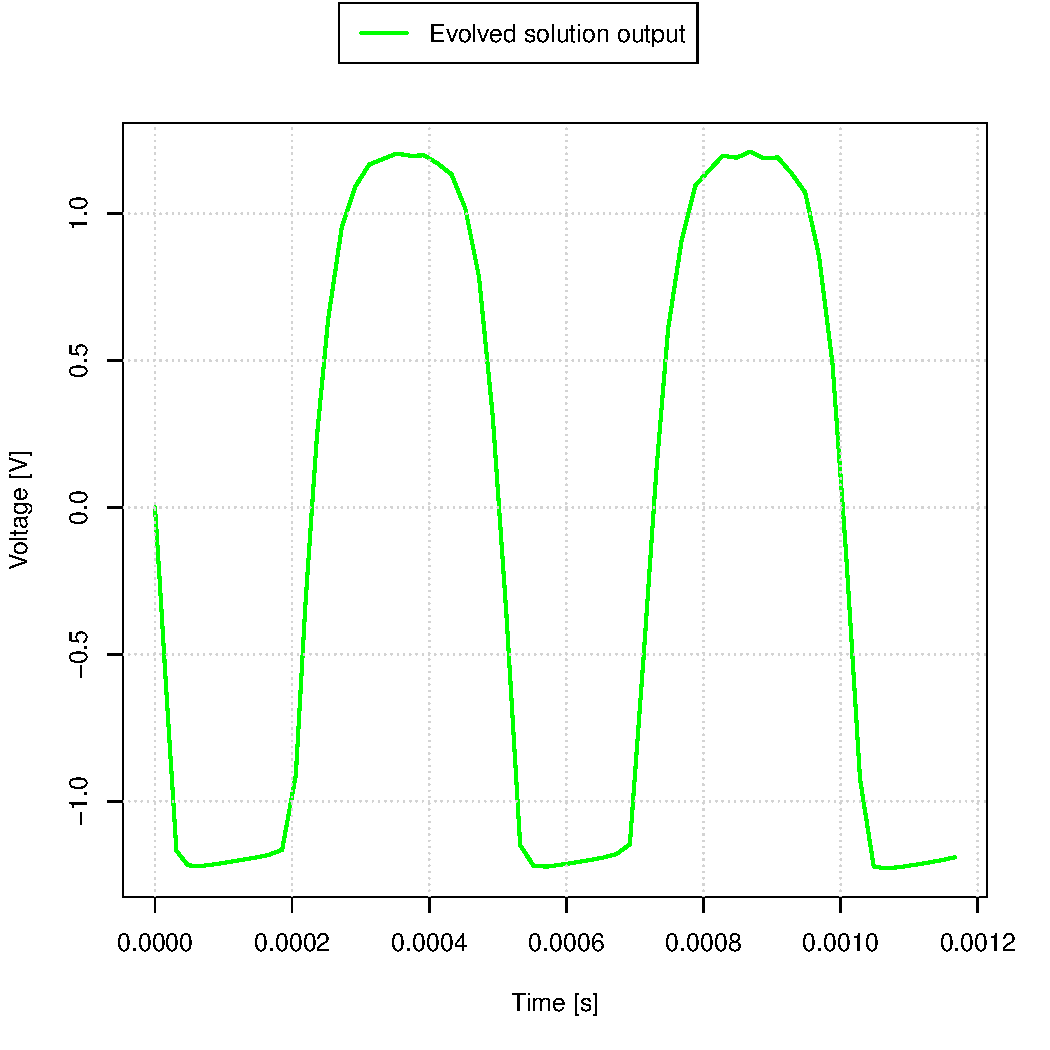
\includegraphics[scale=0.6]{symmetrical-ideal-sine}\label{symmetrical-ideal-sine}}
    \caption{A distorted result using the 'ideal sine wave' evaluation}
\end{figure}

The ability of the evolution to find the desired solution was also decreased because some asymmetrical candidate solutions head towards a good solution. These consequences led to another solution to this problem.

\begin{algorithm}
\caption{Rating the chromosomes with regard to the symmetry of the signal}
\label{symmetry-rating}
\begin{algorithmic}[1]
    \Function{rateChromosome}{$candidateVector$, $maxDifference$}
    \State $min \gets \min(|trough|$, $peak)$;
    \State $max \gets \max(|trough|$, $peak)$;
    \If{\scalebox{1.1}{$\frac{min}{max} < (1 - \frac{maxDifference}{100})$}}
        \State \Return $DOUBLE\_MAX$;
    \EndIf
    \LineComment{continue evaluating the chromosome}
    \EndFunction
\end{algorithmic}
\end{algorithm}

Condition on line 4 in algorithm \ref{symmetry-rating} is used to separate the symmetrical and asymmetrical chromosomes. The values of the variables $trough$ and $peak$ are obtained in the same way as in algorithm \ref{maxAmp}. The value of $maxDifference$ is in the interval $\left[0, 100\right]$ and it is set by the user. It represents the maximal percentage difference between the peak and trough in the second period of the signal. The algorithm calculates the ratio between the peak and trough and if the result is less than the threshold value, the chromosome is evaluated with the maximal fitness and the function is terminated. Otherwise, the evaluation continues. This allows the user to control the results of the evolution with respect to the symmetry of the output signal.

\section{Results}
The results of the experiments discussed below are related to the evolutionary algorithm itself. The results of the optimization of the amplifiers are analyzed in sections \ref{single-stage-results} and \ref{2stage-results}.

\subsection{Initial stages of experiments}
The first experiments were performed only in order to optimize the value of resistor $R1$ in the single stage amplifier. We used the 'best match' evaluation method and mutations with one step size. The evolution always found a value close to \SI{50}{\kilo\ohm} which was the desired solution. These experiments were always successful as this was a very simple task for the evolution.\\
In the next stage, the task was to optimize the voltage divider constituted by $R1$ and $R2$. We again used the 'best match' method and mutations with one step size and it emerged, that the evolution was able to find the solution even faster than in the previous case. This was because we were looking only for the right ratio between the resistors and not for specific values so the set of the desired solutions was larger in this case.\\
The next task for the evolution was to find the right values for resistors $R1$, $R2$ and $Rg$. The evolution parameters were set in the same way as in the previous experiments. This task showed the weak spot of mutations with one step size as the evolution was able to find an acceptable solution very rarely. The reason was that the desired value of $Rg$ is very close to the lower bound of the search space (the analytical value is only \SI{40}{\ohm}). Since mutations with one step size use the same mutation value in every dimension, it was not possible to mutate $Rg$ only by a few ohms (not to move away from the lower bound of this dimension) and at the same time look for the right values in other dimensions which required steps in kiloohms. The value of $Rg$ heavily influences the overall fitness of the chromosome because high values significantly decrease the gain of the amplifier. The usual course of the evolution was that the value of $Rg$ converged quickly to the lower boundary and since this parameter has a great influence on the fitness, the evolution preferred chromosomes with this property. This led to a quick decrease of the mutation step size $\sigma$ (the fitness function also indirectly evaluates the value of $\sigma$) and the algorithm got stuck in a local optimum since other dimensions (values of other resistors) in the search space could not be searched properly. The solution to this problem was to implement mutations with $n$ step sizes discussed in section \ref{n-step}. This approach allows us to treat every dimension separately and therefore search the search space more effectively. After the implementation, the evolution was able to find a satisfactory solution in most of its runs.\\
The previous experiments proved that the evolutionary algorithms are able to provide acceptable solutions in the domain of analog amplifiers. The next section describes the process of determining the ideal parameters for the evolution.

\subsection{Evolution parameters}
In order to make the evolution strategies work efficiently, we need to find and set the correct parameters for the evolution.\\
The size of the search space is defined by the number of dimensions and by the size of every dimension. The number of dimensions depends on the number of electronic components that we want to optimize and the sizes of the dimensions depend on the range the of values that every component can have. These ranges were set from \SIrange{0}{200}{\kilo\ohm} for resistors and from \SIrange{0}{500}{\micro\farad} for capacitors. The upper bounds are based on the values of real electronic components so, for example, we do not expect to have a higher resistance than \SI{200}{\kilo\ohm} in the circuit. The values of some particular components could have a smaller range, for example, resistor $Rg$ which value does not need to be higher than a few kiloohms, but the assumption is that we have no knowledge about the circuit at all.\\
The initial mutation step size $\sigma$ is set to 100. This value is not very important because this parameter is adapted during the evolution. Experiments showed that there is no difference between setting the initial $\sigma$ to 10 or 500 for example. However, if we set the initial value too high (10000 and above), it is more likely that the evolution will get stuck in a local optimum because the algorithm converges too quickly at the start.\\
The experiments also showed that the values of the learning parameters $\tau$ and $\tau'$ have a significant impact on the speed at which the evolution converges to the optimum. The higher the values were, the faster the evolution converged, nevertheless this also means that the probability of finding only a local optimum was rapidly increased. For this reason, the values were set according to formulas \ref{set-tau} and \ref{set-tau-prime} to their lowest possible values. The parameter $n$ is the number of dimensions of the search space.

\begin{equation} \label{set-tau}
    \tau = \frac{1}{\sqrt{n}}
\end{equation}

\begin{equation} \label{set-tau-prime}
    \tau' = \frac{1}{\sqrt{2\sqrt{n}}}
\end{equation}

The maximum difference between the peak and trough of the amplifier's output waveform was empirically set to 25. This means that the values of the peak and trough of the waveform can differ at most by 25 \%.

\subsection{Population size, selection type and selective pressure}
Important parameters of the evolution are numbers $\mu$ and $\lambda$ which define the population size (the number of parents and children in every generation), the ratio between them which defines the selective pressure, and also the type of the selection that we choose for the evolution(($\mu$, $\lambda$)-ES or ($\mu + \lambda$)-ES). In order to determine the most suitable values of the parameters, there were various experiments carried out which are summarized in table \ref{experiments-results}.\\
Every row of the table contains results for a different combination of $\mu$ and $\lambda$. The values of $\mu$ are set to 1, 5, 10 and 15 and the selective pressure is also 1, 5, 10 and 15 for every value of $\mu$, so there are four different values of $\lambda$ for every $\mu$. For every such combination, there are results for both selection types and under every type, there are three columns representing the results of experiments for all the three evaluation methods that are discussed in section \ref{chromosomes-evaluation}. One cell of the table corresponds to the result of one experiment in which the evolutionary algorithm was run 10 times with the same parameters and the fitness values of the best chromosomes were added up and divided by 10. The task was to optimize the single stage amplifier.\\
We can see that there is no significant difference between the selection schemes, provided the selective pressure is higher than one. On lines 5, 9 and 13 (where the selection pressure is 1) the ($\mu$, $\lambda$)-ES scheme performs significantly worse than the ($\mu + \lambda$)-ES scheme and even increasing the population size has no effect (line 5 compared to line 9 and 13). However, when we sum up all the values in both schemes (excluding lines 1, 5, 9 and 13), the latter one gives us better results, so the ($\mu + \lambda$)-ES selection scheme was chosen as the more effective one.\\
We can also see that when the value of $\mu$ is only 1, the algorithm's results are substantially worse than in the rest of the table and on the other hand when we increase it from 5 to 15, there is only a small change in the overall performance.\\
The value of $\lambda$ is set according to the value of $\mu$ and selection pressure and it highly influences the overall computation time of the algorithm because it defines the number of chromosomes that have to be evaluated in every generation (the evaluation includes the amplifier's simulation which takes most of the computation time). When the selective pressure and the value of $\mu$ are higher than one, the overall efficiency of the algorithm does not increase rapidly but there is a noticeable increase in the computation time. For this reason, the values of $\mu$ and $\lambda$ were set to $\mu = 15$ and $\lambda = 150$ as a compromise between the algorithm's time requirements and the optimization efficiency. Also, higher values were examined but they did not provide any significant improvements.

\begin{table}[H]
\centering
\begin{tabular}{@{}ccccccccc@{}}
\toprule
    &       &           & \multicolumn{3}{c}{($\mu$, $\lambda$)-ES} & \multicolumn{3}{c}{($\mu + \lambda$)-ES} \\
   \cmidrule(lr){4-6} \cmidrule(lr){7-9}
    & $\mu$ & $\lambda$ & best match & ideal sin & max. ampl.       & best match & ideal sin  & max. ampl.     \\
   \midrule
1.  & 1     & 1         & N/A        & N/A       & N/A              & 21.82      & 99.00      & 2.90           \\
2.  & 1     & 5         & 20.82      & 113.75    & 1.98             & 13.44      & 57.91      & 2.69           \\
3.  & 1     & 10        & 18.84      & 76.81     & 1.40             & 24.70      & 75.01      & 2.84           \\
4.  & 1     & 15        & 18.43      & 128.75    & 2.26             & 19.52      & 34.11      & 1.02           \\
5.  & 5     & 5         & 49.62      & 169.02    & 36.50            & 9.81       & 56.61      & 3.18           \\
6.  & 5     & 25        & 7.28       & 55.00     & 3.12             & 12.12      & 34.88      & 2.72           \\
7.  & 5     & 50        & 16.18      & 64.22     & 3.21             & 9.75       & 43.73      & 3.57           \\
8.  & 5     & 75        & 3.70       & 58.82     & 3.10             & 4.20       & 38.84      & 3.52           \\
9.  & 10    & 10        & 49.41      & 154.66    & 26.40            & 8.94       & 53.77      & 3.18           \\
10. & 10    & 50        & 9.09       & 60.93     & 2.68             & 7.02       & 45.04      & 3.58           \\
11. & 10    & 100       & 6.97       & 38.02     & 3.16             & 4.91       & 26.06      & 3.10           \\
12. & 10    & 150       & 8.06       & 25.54     & 3.10             & 2.52       & 23.07      & 3.07           \\
13. & 15    & 15        & 44.48      & 165.76    & 34.99            & 2.54       & 47.69      & 3.18           \\
14. & 15    & 75        & 4.64       & 56.18     & 2.25             & 4.96       & 51.74      & 3.56           \\
15. & 15    & 150       & 6.63       & 47.32     & 3.52             & 6.36       & 12.19      & 1.60           \\
16. & 15    & 225       & 7.56       & 31.17     & 2.65             & 0.70       & 19.31      & 1.08           \\
    \bottomrule
\end{tabular}
\caption{Experiments results}
\label{experiments-results}
\end{table}


All the evolution parameters discussed above are summarized in table \ref{evolution-parameters}. These parameters were chosen as the most appropriate ones.

\begin{table}[H]
\centering
\begin{tabular}{@{}ll@{}}
\toprule
    Parameter                   & Value \\ \midrule
    Resistance range            & \SIrange{0}{200}{\kilo\ohm} \\
    Capacitance range           & \SIrange{0}{500}{\micro\farad} \\
    initial $\sigma$            & 100 \\
    max. peak-trough difference & 25 \% \\
    $\mu$                       & 15 \\
    $\lambda$                   & 150 \\
    selection type              & ($\mu + \lambda$)-ES \\
    $\tau$                      & equation \ref{set-tau}\\
    $\tau'$                     & equation \ref{set-tau-prime} \\ \bottomrule
\end{tabular}
\caption{Evolution parameters}
\label{evolution-parameters}
\end{table}

\subsection{The typical course of the evolution}
Figure \ref{evolution-course} shows us the typical course of the evolution. The population size parameters were set to $\mu = 10$ and $\lambda = 100$ and the terminating condition of the algorithm was that the evolution ends when the value of the fitness function of the best chromosome does not change by more than 1\% after 300 generations.\\
The green line represents the fitness of the best chromosome (the one with the lowest fitness) in every generation, the blue line is the fitness of the worst chromosome and the red line is the average fitness of every generation. In this case, we pick the chromosomes only from the set of $\mu$ parents. We can see that the red line is very close to the green line so the average fitness of every generation is close to the fitness of the best chromosome and that the blue line is scattered above the green line. The evolution was stuck in a local optimum for approximately 20 generations between the 80th and 100th generation and the solution was evolved approximately after 300 generations. When the blue line is close the other two lines, it means that the sizes of the mutation steps $\sigma$ are low and the algorithm searches only a small area of the search space. When the values of $\sigma$ are low (close to zero), we can stop the algorithm after a few hundreds of generations because it will not provide any better solution than the current one and the resulting fitness is either in a local or global optimum. The usual amount of generations after which the fitness does not change anymore is a few hundred. When the size of the population is low (for example $\mu = 1$ and $\lambda = 5$), the optimization takes a few thousands of generations.\\
The evaluation method was the 'best match' method and this evolution run was successful since the resulting fitness was very close to zero. With this method, we can consider those solutions which fitness is under 0.5 as sufficient because the amplifier's output waveform is very close to the desired one. The resulting value of the fitness of the best chromosome was 0.19.

\begin{figure}[H]
    \centerline{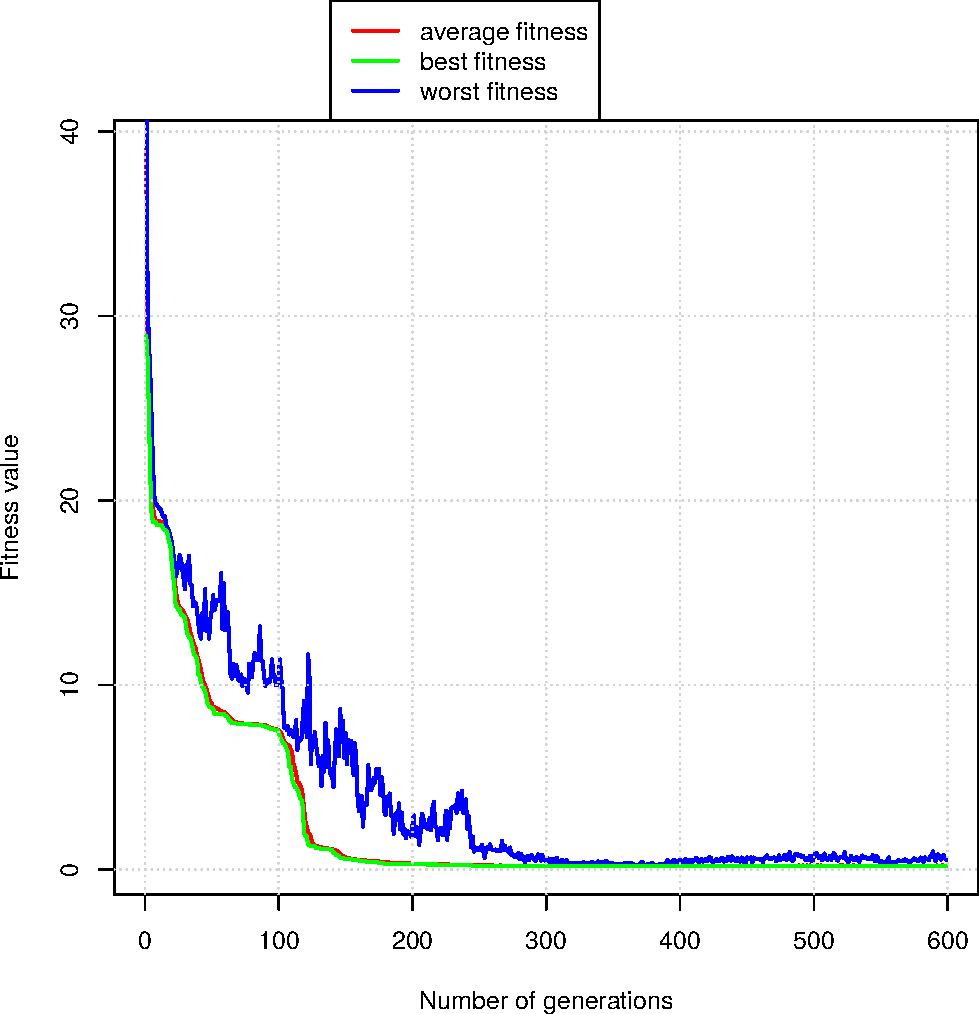
\includegraphics[scale=0.6]{evolution-course}\label{evolution-course}}
    \caption{The typical course of the evolution}
\end{figure}

\subsection{Single stage amplifier optimization} \label{single-stage-results}
Every evaluation method implemented in this thesis provides us different means by which we can optimize the circuit.\\
The 'best match' method can be used for finding such properties that provide us the most similar output compared to the analytical solution. We optimize the values of 8 electronic components and experiments with this method proved that there are many other possible combinations which provide almost identical behaviour of the amplifier. Five examples are shown in table \ref{best-fit-solutions}. The simulation output of the amplifier with these components' values was visually identical with the analytical solution.\\

\begin{table}[H]
\centering
\begin{tabular}{@{}c ccccccc@{}}
\toprule
    $R1$ [\si{\kilo\ohm}] & $R2$ [\si{\kilo\ohm}] & $Re$ [\si{\ohm}] & $Rg$ [\si{\ohm}] & $Rc$ [\si{\kilo\ohm}] & $Ce$ [\si{\nano\farad}] & $Cin$ [\si{\nano\farad}] & $Cout$ [\si{\nano\farad}] \\
    \midrule
    200   & 76.2 & 7510  & 471 & 21.7 & 460     & 29    & 1010 \\
    78.5  & 16   & 3370  & 429 & 23   & 228 000 & 17    & 396 000 \\
    141   & 11.5 & 180   & 483 & 21.1 & 285 000 & 21    & 280 000 \\
    82.3  & 44.3 & 8590  & 400 & 16   & 499     & 202   & 95 \\
    118   & 41.2 & 11500 & 559 & 35.4 & 419     & 95    & 19 \\
    \bottomrule
\end{tabular}
\caption{Solutions similar to the analytical one}
\label{best-fit-solutions}
\end{table}

The 'maximal amplitude' method can be used for finding the best amplification capabilities of the circuit as it does not take into consideration the shape of the output signal. This method is useful for the 'ideal sine' method because it allows us to find the appropriate maximal amplitude and then we can find the right waveform by using the latter method. If we set the amplitude for the 'ideal sine' method too high, it would not work as effectively as when we set some realistic number. By this approach, we can find even better solutions than the analytical one. One of such solutions is shown in figure \ref{better-solution-fig} and the values of the components are summarized in table \ref{better-solution-tab}. Since the amplitude of the input signal was \SI{100}{\milli\volt} and the amplitude of the output signal is approximately \SI{4.2}{\volt}, the gain of this amplifier is approximately 42 (the gain of the analytically solved amplifier is approximately 18).\\

\begin{figure}[H]
    \centerline{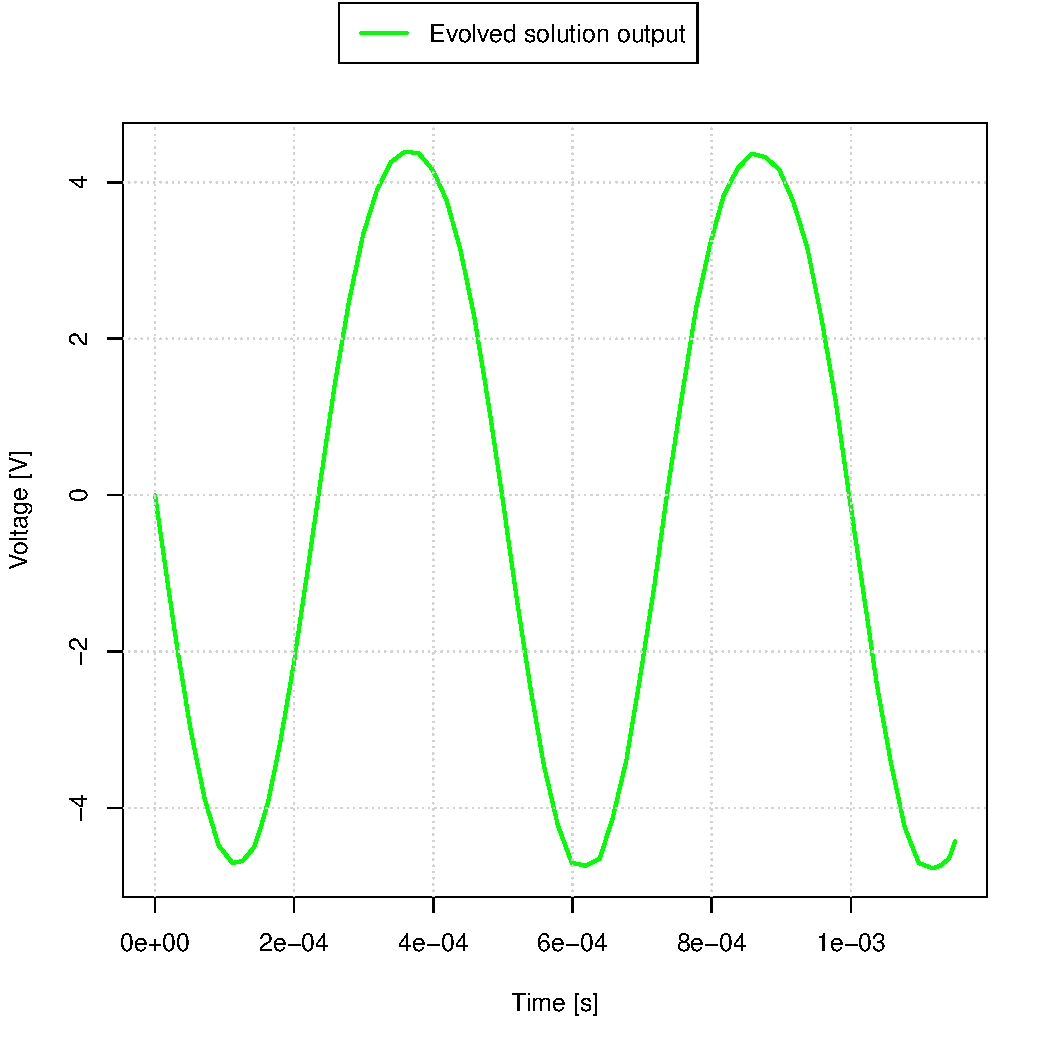
\includegraphics[scale=0.6]{best-solution-single-stage}\label{better-solution-fig}}
    \caption{The best solution}
\end{figure}

\begin{table}[H]
\centering
\begin{tabular}{@{}cccccccc@{}}
\toprule
    $R1$ [\si{\kilo\ohm}] & $R2$ [\si{\kilo\ohm}] & $Re$ [\si{\ohm}] & $Rg$ [\si{\ohm}] & $Rc$ [\si{\kilo\ohm}] & $Ce$ [\si{\micro\farad}] & $Cin$ [\si{\micro\farad}] & $Cout$ [\si{\nano\farad}] \\
    \midrule
    168 & 15.1 & 169 & 49 & 4.21 & 16 & 274 & 86 \\
    \bottomrule
\end{tabular}
\caption{The best solution}
\label{better-solution-tab}
\end{table}

The 'ideal sine' evaluation method also provides us a universal tool for finding the appropriate components' values which produce an arbitrary amplification of the amplifier up to the maximal amplitude.

\subsection{Two stage amplifier optimization} \label{2stage-results}
This amplifier was chosen as the more complicated task to optimize. There was no analytical solution for this circuit so it was not possible to use the 'best match' evaluation method. Experimenting with this type of amplifier showed that this amplifier is much more difficult to optimize and that it does not provide any better amplification properties than the previous single stage amplifier.\\
The same set of experiments was carried out as for the previous amplifier and one of the best solutions is shown in figure \ref{best-solution-two-stage-fig}.\\

\begin{figure}[H]
    \centerline{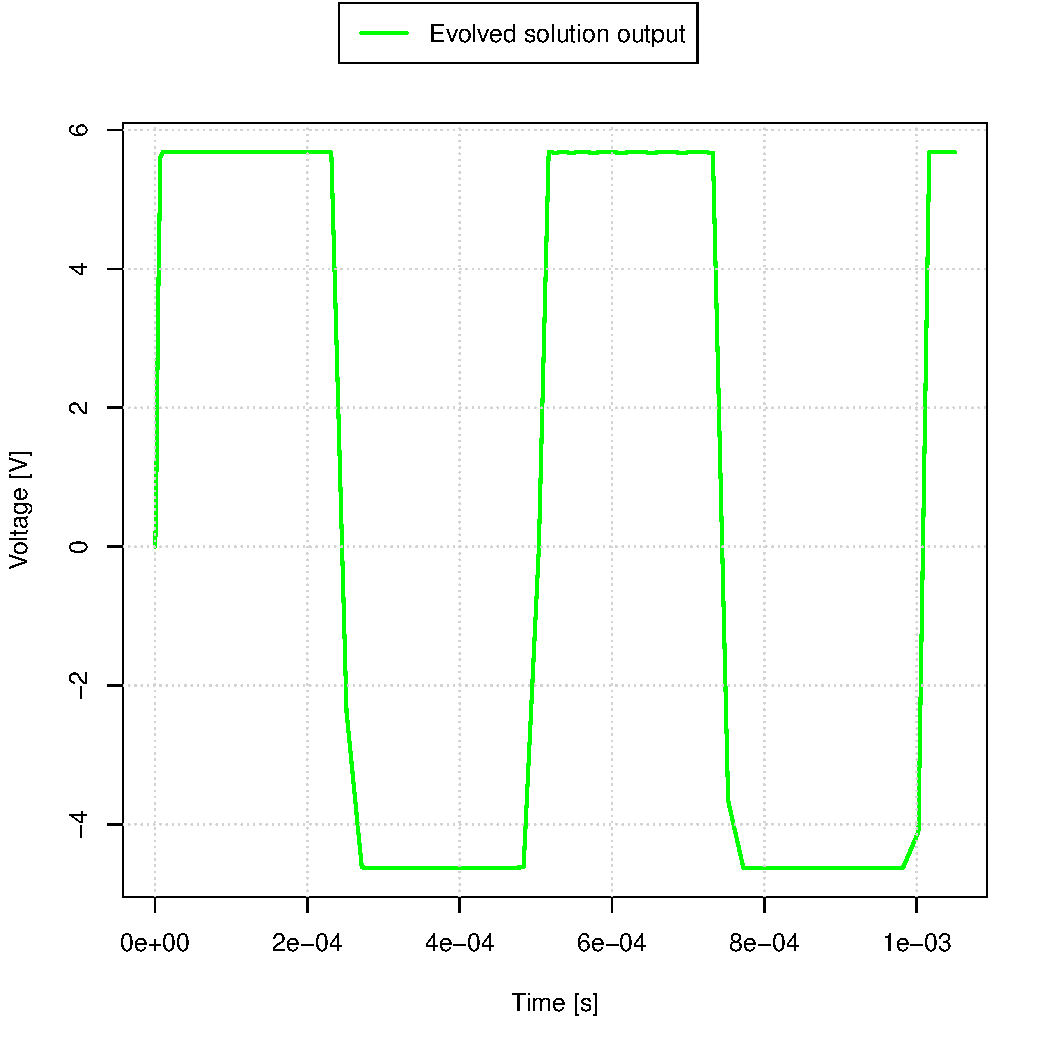
\includegraphics[scale=0.6]{best-solution-two-stage}\label{best-solution-two-stage-fig}}
    \caption{The best solution}
\end{figure}

We can see that the resulting gain is approximately 50 (the amplitude of the input voltage is \SI{100}{\milli\volt}) but the output waveform is significantly distorted --- the circuit generates a square wave. The experiments did not provide any solution that would generate a sine wave. The components' values are stated in table \ref{best-solution-two-stage-tab}.

\begin{table}[H]
\centering
\begin{tabular}{@{}cccccccccccccc@{}}
\toprule
    $R1$ [\si{\kilo\ohm}] & $R2$ [\si{\kilo\ohm}] & $Re$ [\si{\kilo\ohm}] & $Rc$ [\si{\kilo\ohm}] & $Ce$ [\si{\micro\farad}] & $Cin$ [\si{\micro\farad}] & $Cout$ [\si{\micro\farad}] \\
    $Rgb$ [\si{\ohm}] & $Reb$ [\si{\ohm}] & $Rcb$ [\si{\kilo\ohm}] & $R2b$ [\si{\kilo\ohm}] & $R1b$ [\si{\kilo\ohm}] & $Cm$ [\si{\micro\farad}] & $Ce2$ [\si{\micro\farad}] \\
    \midrule
    114 & 57  & 51.6 & 81.7 & 98   & 215 & 479 & \\
    22  & 298 & 3.37 & 9.24 & 80.5 & 351 & 139   \\
    \bottomrule
\end{tabular}
\caption{The best solution}
\label{best-solution-two-stage-tab}
\end{table}